% Paper for Learning-Based Controls (ME 537)

\documentclass[letterpaper, 10 pt, conference]{ieeeconf}  % Comment this line out if you need a4paper

\IEEEoverridecommandlockouts                              % This command is only needed if 
                                                          % you want to use the \thanks command

\overrideIEEEmargins                                      % Needed to meet printer requirements.


%\usepackage{ijcai09}  % style
\usepackage{times}    % font
\usepackage{graphicx} % inserting images
\usepackage{cite}
\usepackage{mathtools} % For math
\usepackage{hyperref}
\renewcommand{\deg}{\ensuremath{^{\circ}}\xspace}  % why doesn't this work???

\providecommand{\e}[1]{\ensuremath{\times 10^{#1}}}

\graphicspath{ {./figures/} } % Point to the figures directory

%%%%%%%%%%%%%%%%%%%%%%%%%%%%%%%%%%%%%%%%%%%%%%%%%%%%%%%%%%%%%%%%%%%%%%%%%%%

\title{\LARGE \bf 
O Rover Where Art Thou?\\
Multi-Robot Exploration with Limited Sensor Field-of-View
}

\author{Kory Kraft$^{1}$, Austin Nicolai$^{2}$, and Matthew Rueben$^{3}$% <-this % stops a space
%\thanks{*This work was supported by... }% <-this % stops a space
\thanks{*All authors are with the School of Mechanical, Industrial, and Manufacturing Engineering,
         Oregon State University,
         Corvallis, OR, USA. }% <-this % stops a space
\thanks{$^{1}$Corresponding author: {\tt\small kraftko@onid.oregonstate.edu}}%
\thanks{$^{2}$Corresponding author: {\tt\small nicolaia@onid.oregonstate.edu}}%
\thanks{$^{3}$Corresponding author: {\tt\small ruebenm@onid.oregonstate.edu}}%
}

\begin{document}

\maketitle
\thispagestyle{empty}
\pagestyle{empty}

\begin{abstract}
We should write one.
\end{abstract}


\section{Introduction}
Robots have been targeted for use in the exploration domain, both in
single agent and multiagent systems.  Robots have the potential to
handle certain extreme environments better than their human
counterparts, and in some cases cover large swaths of territory more
efficiently, or conversely fit in very tight spaces without disturbing
the surrounding environment (e.g. snake robots). Furthermore, the
decreasing cost and increasing capability of computer hardware makes
robots an attractive alternative to human labor.

A number of inroads have been made into harnessing the power and
advantages of robots in the exploration domain.  NASA continues to use
the rover Curiosity to explore Mars.  Several companies have built
mobile robots to explore and decontaminate the the Fukushima Daiichi
nuclear power station after the 2011 meltdown CITE THE URL. Added to these
accomplishments, robots are increasingly being used in conjunction
with one another, giving added significance to multiagent systems
(MAS) studies.

Previous MAS research however, often fails to consider the effect of
sensor limitations upon the learning algorithm by (perhaps implicitly)
assuming that the sensor range is large compared to the search space.
In many realistic cases, however, the sensor falls quite short of
being able to see the entire search space at once. Many lower-cost
robots are now using the Microsoft Kinect because it offers RGB-D
sensing for fewer than 100, albeit with a 0.8 - 4.0m effective range
and significant sensor noise.

We will show the trade-offs between using more robots with
limited-range sensors and using fewer robots with costlier
sensors. This includes analyzing the effect of sensor range, noise,
and field of view, as well as the number of robots and different
multi-agent learning algorithms, on performance in an arbitrary
exploration task. This will help future implementers conduct more
accurate cost-benefit analyses in order to make wiser decisions when
building and deploying robotics in the real world.

Here's a sample figure: Figure~\ref{fig:ATRIAS}. Here's a sample
citation \cite{nuclear_robots}.

\begin{figure}[h!]
    \centering
    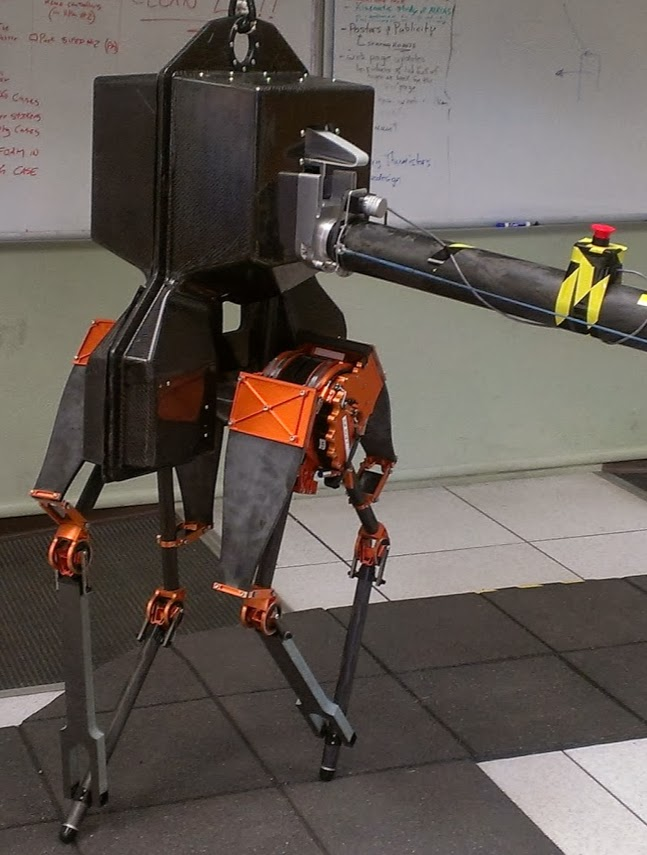
\includegraphics[width=0.3\textwidth]{ATRIAS.jpg}
    \caption{A sample figure, this being the sample caption for the sample figure.}
    \label{fig:ATRIAS}
\end{figure}

Here's a sample equation:
\begin{align*}
    m\ddot{x} &= F_x
\\  m(\ddot{y}+g) &= F_y
\\  I\ddot{\theta}_T &= X_{vpp}(F_x cos(\theta_T+\theta_{vpp})-F_y sin(\theta_T+\theta_{vpp}))
\end{align*}


\section{Related Work}
\subsection{Continuous Rover Domain}
Blah blah blah?

\subsection{Congestion}
One unique aspect of a multi-agent system is the congestion
problem. In the domain of search and retrieval tasks, it was shown
that increasing the number of agents present, up to a saturation
point, increases the overall system performance and speed. However, at
some point, additional agents provide no extra benefit due to
congestion of the experimental space \cite{rybski1998performance}. The challenge of
reward-shaping has been examined in a noisy domain involving
competitive robotic “foraging”. It was shown that intelligent
reward-shaping and algorithm use was required to overcome the distinct
challenges presented by the dynamic environment and achieve good
performance \cite{mataric1997reinforcement}.

\subsection{Credit Assignment}
A second unique aspect of a multi-agent system is the problem of
credit assignment. Agent to agent coordination involves individual
agents working together on a common task or goal.  Since one agent’s
behaviors might affect other agents, however, the learning process
becomes hard. Chalkiadakis and Boutilier \cite{chalkiadakis2003coordination} develop a way to weigh
the costs and benefits of taking non-greedy actions during
reinforcement learning based on the value of the new information that
might be gained. They also give the agents some limited ability to
reason about how their actions influence others. Another question is,
what does each agent know about the other agents? This is the
information by which they can coordinate at all. Gmytrasiewicz and
Durfee \cite{gmytrasiewicz2000rational} expand the typical state space of each agent by adding
knowledge about other agents’ knowledge, which is recursive by
nature. They develop a framework whereby this representation is
usable, however, and present their findings as a move towards
coordinated robot actions. Finally, Burgard et al. \cite{burgard2005coordinated} address
coordination in an exploration scenario, which for them boils down to
intelligently placing goal locations (or waypoints, by extension) for
each agent.

\subsection{Exploration Domain}
In the exploration domain, agents must discover all areas of an
initially unknown map. One method tackles the search of complicated
areas via cellular decomposition and systematic coverage \cite{choset2001coverage}. Another
method examines the effect of limited knowledge on an agent. It
examines how well different algorithms utilize agents, as well as how
the number of rooms and room size effects the explorability of a space
\cite{ferranti2007brick}. Lastly, one method coordinates exhaustive exploration of a space
by intelligently assigning destinations to different agents \cite{burgard2005coordinated}.

\subsection{Sensor Limitations}
A limited sensor range causes two potential problems for agents:
collision with each other and sub-optimal behavior due to lack of
coordination. Dimarogonas et al. \cite{dimarogonas2007decentralized} and Do \cite{do2007bounded} present planning
approaches to collision avoidance with limited sensor range. To plan
agent motion, both approaches use potential fields (also called
navigation functions) that include some potential or proximity
function between each pair of agents that can see each other. The ant
colony problem presented by Gordon et al. \cite{gordon2004gathering} examines the case where
the sensors have limited range and no distance information, i.e., only
output the direction to sensed entities. All of these approaches
involve sending the agents to some goal location or formation, not
exploring an area, and no machine learning techniques are used.

\subsection{Noise}
Blah blah blah?


\section{Methods}
\subsection{Domain}
This work is a direct extension of that described by Tumer and Agogino
(2008, \cite{agogino2008analyzing}). Therein, the goal of the rovers is to observe the more
important points of interest (POIs) at close range in order to earn a
large reward. We use their dynamic domain rather than their static
domain, so the POI values and locations are chosen randomly at the
beginning of each learning episode. For each learning episode, the
rovers begin in a tight cluster at the center of the map. The episode
ends after 15 time steps and rewards are assigned. Each rover can move
continuously in two dimensions, and 10 percent noise is added to the
intended movement to simulate real-world errors.

\subsection{Reward Structure}
The global reward presented by Tumer and Agogino (2008) is based on
the closest observation of each POI by any rover:
  
\[
G= \sum_j  \frac{V_j}{min_i \: \delta(L_j, L_i)}
\]

The distance function is the square of the Euclidean norm up to a
minimum distance d2:

\[
\delta  (x,y) = max \big\{||x - y||^2, d^2 \big\}    
\]

The difference reward would be more learnable for an individual rover,
but requires each rover to calculate the hypothetical global reward if
that rover were removed from the system. For this work, we use the
partial observation difference reward, which only accounts for the
rover in question and any rovers within its sensor range. If a rover
is the closest rover that it knows of to a given POI, it is credited
with the reward for that POI:

\[
D_i(PO) = \sum_j  \frac{V_j}{min_{i' \in O^\rho_i} \: \delta(L_j, L_{i'})} - \sum_j  \frac{V_j}{min_{i' \in O^\rho_i,  \neq i} \: \delta(L_j, L_{i'})}
\]

The authors showed this to be a highly factored, learnable, and
practical credit assignment structure.

\subsection{State Information}
Each rover has two types of sensors. The first type returns an
aggregate score that represents how many high-value POIs are near the
rover:

\[
s_{1,q,i} =  \sum_{J \in I_q}  \frac{V_j}{\delta (L_j, L_i)} 
\]

The second sensor type returns a similar aggregate for other rovers:

\[
s_{2,q,i} =  \sum_{i' \in N_q}  \frac{V_j}{\delta (L_{i'}, L_i)}  
\]

Each rover’s surroundings are divided into four quadrants and two
sensors -- one POI sensor and one rover sensor -- look out on each
quadrant. Eight total sensors therefore yield eight continuous state
variables.

\subsection{Action Selection and Learning}
State information was mapped to action choices using a perceptron with
8 inputs, 10 hidden nodes, and 2 outputs. The activation functions
were sigmoidal and each output value was scaled based on a maximum
movement allowance per step (d is maximum movement per time step and
o1, o2 are the perceptron outputs):

\[
dx = 2d(o_1-0.5)
\]
\[
dy = 2d(o_2-0.5)
\]

An evolutionary algorithm was used with simulated annealing to find
neural networks that yield good performance. This is called “direct
policy search” because we use an evolutionary algorithm to search for
a good policy directly, i.e., without maintaining state-action value
estimates as in approaches like Q-learning. The system described thus
far provides the basis for our study of sensor limitations. Our novel
study regarding sensor impact is detailed below.

\subsection{Sensor Evaluation}
Sensor impact upon learning was evaluated by comparing the baseline
system performance from \cite{agogino2008analyzing} with the system performance after limiting
the sensors in three ways: reducing range, adding noise, and reducing
the field-of-view angle.  Following \cite{agogino2008analyzing}, we defined system performance
as the sum global reward achieved.  Noise was defined as the random
error in a rover’s distance measurements. All three types of sensor
limitations were applied to the POI sensors and the rover sensors
equally. Due to the 2D nature of the simulated world, height was
ignored and sensor field-of-view angle was only measured about the
vertical axis.

Each sensor limitation was applied independently at three different
magnitudes.  Thus, we had 9 test cases total plus the 1 baseline
case. The baseline sensor combination was chosen after \cite{agogino2008analyzing} as having
unlimited sensor range, zero noise, and a 360° field of view. Sensor
range was tested at 1 world unit, 3 world units, and unlimited world
units. Sensor noise was modeled as a unique normal distribution for
each sensed object with standard deviations at 0\%, 10\%, and 30\% of the
object’s true range. Sensor viewing angles were tested at 90$^{\circ}$, 270$^{\circ}$,
and 360$^{\circ}$.

100 statistical system runs were executed for 1000 episodes for each
sensor combination at three separate scales: 10, 50, and 100
homogeneous agents.  System performance was then plotted for each
sensor attribute at each scale in comparison with the baseline sensor
performance.



\bibliographystyle{IEEEtran}
\bibliography{main}


\end{document}
